\begin{center}
  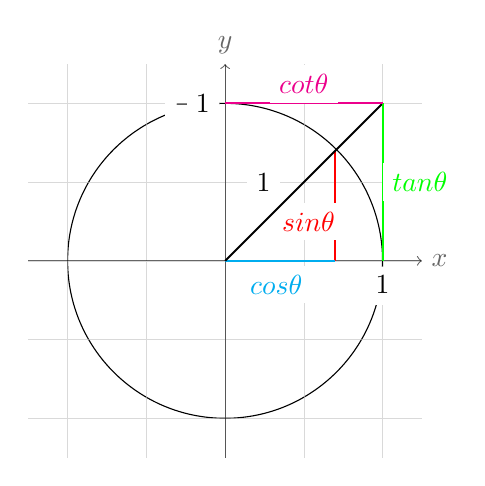
\begin{tikzpicture}
    %circle
    \draw[smooth, samples = 600] (0, 0) circle (2)(1, 1);
    
    % coordinate system
    \draw[opacity=0.6,lightgray,very thin,step=1cm](-2.5,-2.5) grid (2.5,2.5);
    \draw[->,opacity=0.6](-2.5,0) -- (2.5,0) node [right]{$x$};
    \foreach \x in {-1,...,1}
    \draw[xshift=2cm] (0,2pt) -- (0,-2pt) node[below,fill=white]{$\x$};
    \draw[->,opacity=0.6](0,-2.5) -- (0,2.5) node[above]{$y$};
    \foreach \y in {-1,...,1}
    \draw[yshift=2cm] (2pt,0) -- (-2pt,0) node[left,fill=white] {$\y$};
    
    %sin
    \draw[line width=0.25mm,red] (1.39, 1.39) -- (1.39,0);
        \draw (0.6,0.5) node[red,right,fill=white] {$sin\theta$};
    %cos
    \draw[line width=0.25mm,cyan] (0, 0) -- (1.39, 0);
        \draw (0.65,-0.3) node[cyan,fill=white] {$cos\theta$};
    %Hypotenuse
    \draw[line width=0.25mm,black] (0, 0) -- (2, 2);
        \draw (0.7,1) node[left, black,fill=white] {$1$};
    %tan
    \draw[line width=0.25mm,green] (2,0) -- (2, 2);
        \draw (2, 1) node[green, right, fill=white] {$tan\theta$};
    %cot
    \draw[line width=0.25mm,magenta] (2, 2) -- (0, 2);
        \draw (1, 2) node[magenta, above, fill=white] {$cot\theta$};
    
  \end{tikzpicture}
\end{center}